\documentclass[aspectratio=169]{beamer}
\usetheme{Copenhagen}
%% Remove draft for real article, put twocolumn for two columns
\usetheme{metropolis}
\usepackage{multicol}
\usepackage[style=british]{csquotes}

\def\signed #1{{\leavevmode\unskip\nobreak\hfil\penalty50\hskip1em
  \hbox{}\nobreak\hfill #1%
  \parfillskip=0pt \finalhyphendemerits=0 \endgraf}}

\newsavebox\mybox
\newenvironment{aquote}[1]
  {\savebox\mybox{#1}\begin{quote}\openautoquote\hspace*{-.7ex}}
  {\unskip\closeautoquote\vspace*{1mm}\signed{\usebox\mybox}\end{quote}}

\usepackage[utf8]{inputenc}
\newtheorem*{question}{Question}

\newcommand{\vectorproj}[2][]{\mathrm{proj}_{\vect{#1}}\vect{#2}}
\newcommand{\vectorcomp}[2][]{\mathrm{comp}_{\vect{#1}}\vect{#2}}
\newcommand{\vect}{\mathbf}
\newcommand{\R}{\mathbb{R}}
%% commentary bubble
\newcommand{\SV}[2][]{\sidenote[colback=green!10]{\textbf{SV\xspace #1:} #2}}

\title{ Multivariable Calculus \\  Optimization }
\date{06/03/2024}

\begin{document}

\maketitle

\begin{frame}
    \frametitle{Quiz}
    What is the difference between derivative and gradient of a function $f:\R^n \to \R$?
\end{frame}



\begin{frame}
    \frametitle{Optimization: Motivations}
    \begin{aquote}{Leonhard Euler}
    Nothing takes place in the world whose meaning is not that of some maximum or minimum.
    \end{aquote}
    \url{https://www.youtube.com/watch?v=IHZwWFHWa-w}
\end{frame}

\begin{frame}
    \frametitle{Motivations}
    \begin{itemize}
        \item Economics
        \item Data analysis
        \item Machine learning 
        \item Physics
        \item Even the stuff that seems the most random like flipping a coin (and Brownian motion) 
            comes from an optimization problem!
    \end{itemize}
\end{frame}


\begin{frame}
    \frametitle{Some toy problems: Economics}
       A store tries to optimize its sale of Apple Macbook Air and Lenovo Thinkpad.  
       A Macbook Air has the retail price $\$1000$ and a Thinkpad $\$700$.
       The importation costs for the two laptops would be $\$900$ for the Macbook Air and
       $\$500$ for the Thinkpad.
       The initial capital of the store is $\$100,000$. 

       How many Macbook Airs and Thinkpads should the store import if it wants to optimize its profit?
\end{frame}

\begin{frame}
    \frametitle{Some toy problems: Data analysis}
    Suppose a scientist has a collection of paired data $\{ (x_i, y_i)\}_{i=1}^N$.
        What is the formula for line that ``best fits'' with the data?
\end{frame}

\begin{frame}
    \frametitle{Some toy problems: Machine learning}
    What is the best label for the following?

    \includegraphics[width = 0.5\textwidth]{cat.jpeg}
    \pause

    (Cat)
\end{frame}

\begin{frame}
    \frametitle{Some toy problems: physics}
    Fermat's principle: light takes path that minimizes the time it travels.

    What is the path?
\end{frame}


\begin{frame}
    \frametitle{Some toy problems: information theory}
    A long string of characters is picked from the 26 alphabets.

    How should we distribute the alphabets so that the string looks as chaotic as possible?
    \pause

    Claude Shannon's proposal: use the entropy function
    \begin{equation*}
        - \sum_{i=1}^{26} p(x_i) \log (p(x_i)) \,,
    \end{equation*}
    where $x_i$ is the $i$th alphabet and $p(x_i)$ is the probability that $x_i$ 
    will appear at random.
    This measures how chaotic a certain probabilistic behavior could be.

    \url{https://people.math.harvard.edu/~ctm/home/text/others/shannon/entropy/entropy.pdf}

    \url{https://www.youtube.com/watch?v=v68zYyaEmEA}
\end{frame}

\begin{frame}
    \frametitle{Caution}
    The field of optimization as a whole is a very old field.
    However, regardless of its long history (over 200 years now, since Newton),
    there's not much one could do when it comes to real life. 

    There are a lot of questions still remained open in this field. 

    The ``most approachable'' kind of optimization is called \emph{convex optimization}. \pause
    
    People manage to study this without differentiability conditions. \pause

    People also use techniques in convex optimization to study 
    non-convex optimization, which is still an untamed beast.
\end{frame}

\begin{frame}
    \frametitle{Let's start with the basics, when everything is nice...}
    Question: what way do you go when you climb a mountain?

    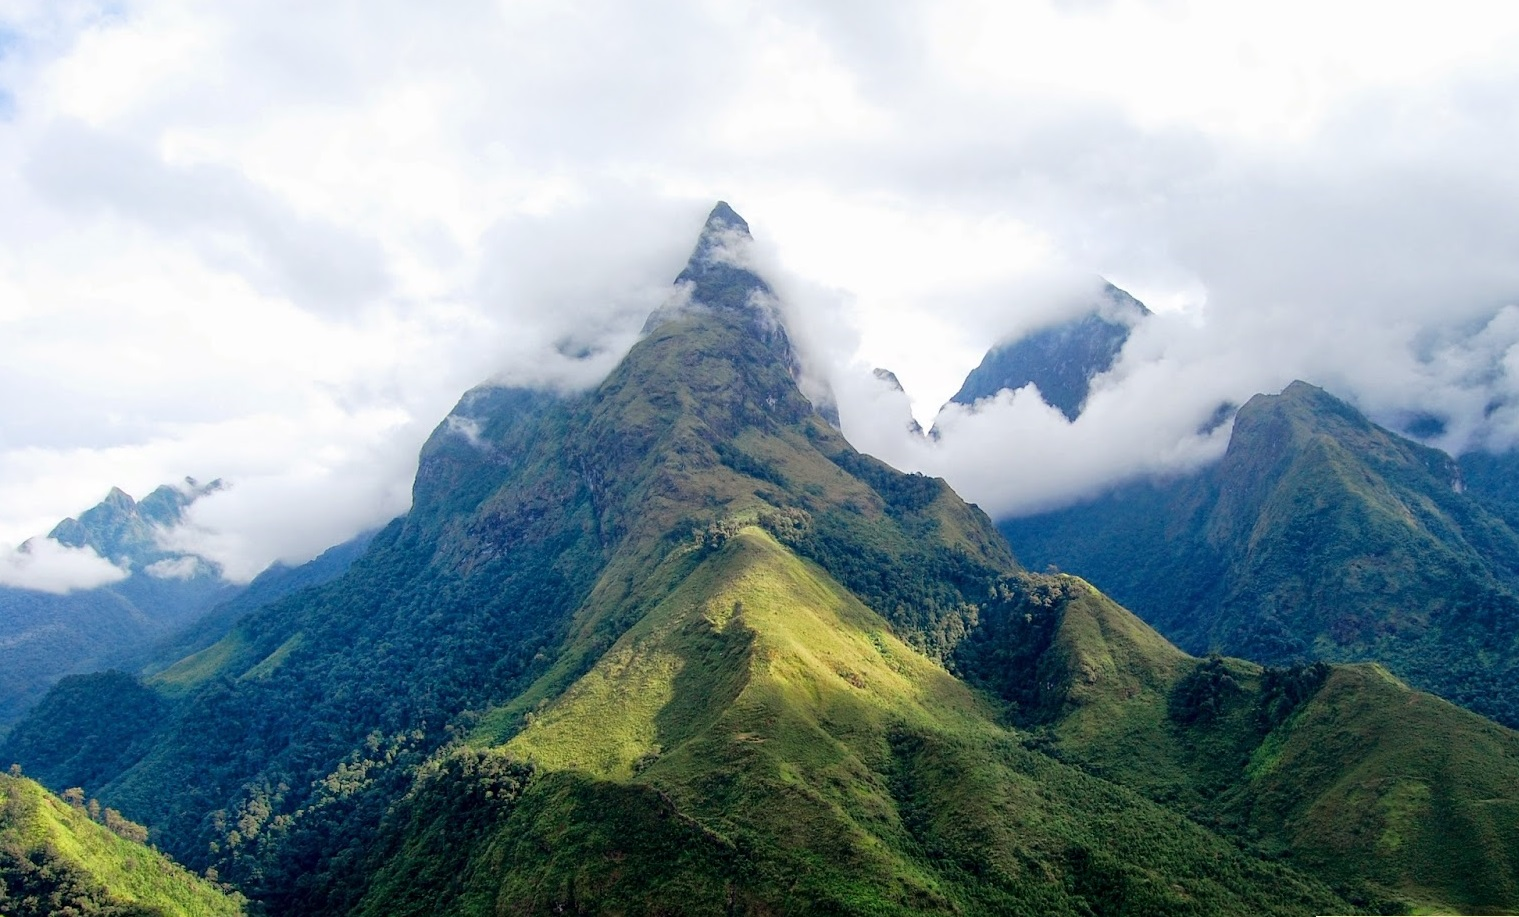
\includegraphics[width = 0.6\textwidth]{fansipan.jpg} 

\end{frame}

\begin{frame}
    \frametitle{Basics}
\begin{definition}
A function \(f:D \to \mathbb{R}\) has a \textbf{local maximum} at \(\mathbf{x_0}\) if
\(f(\mathbf{x_0}) \geq f(\mathbf{x})\) for \(\mathbf{x} \in B_\delta(\mathbf{x_0})\) for small enough \(\delta\).
\(f\) has a \textbf{global maximum} at \(\mathbf{x_0}\) if
\(f(\mathbf{x_0}) \geq f(\mathbf{x})\) for \(\mathbf{x} \in D\).
\(f\) has a \textbf{local (global) minimum} at \(\mathbf{x_0}\) if
\(-f\) has a local (global) maximum at \(\mathbf{x_0}\)
\end{definition}

\end{frame}


\begin{frame}
    \frametitle{A necessary condition}
\begin{theorem}[First derivative test]
Let \(f:D \to \mathbb{R}\) be a function.
If \(\mathbf{x_0}\) is a local minimum and \(f\) has partial derivatives at \(\mathbf{x_0}\).
Then
\begin{equation*}
    \partial_{x_i} f(\mathbf{x}_0) = 0 \,.
\end{equation*}
\end{theorem}
\end{frame}


\end{document}

